\section{Simulation Results}
\label{sec:results}

\subsection{The first honest night}

Figures \ref{fig:fig01_balanced_cycle_event} and \ref{fig:fig02_first_night_accounting} begin with the exact accounting of the first honest night, because every later inequality result inherits its force from that local break. Figure \ref{fig:fig01_balanced_cycle_event} traces the honest agent, the predecessor, the successor, and the remaining population in event time. The pattern is exactly the one derived in Lemma \ref{lem:first-night}. The honest agent does not suffer an immediate loss because he is at home on the first night. The predecessor who attempts to rob that occupied house receives no loot and is still robbed by his own predecessor, so his wealth falls. The successor, who would otherwise have been robbed by the honest agent, keeps the proceeds of his own raid and receives the first windfall. The initial rupture therefore takes the form of a precise redistribution within a three agent neighborhood of the original cycle.

\begin{figure}[tbp]
    \centering
    
\includegraphics[width=\mainfigwidth]{figures/fig01_balanced_cycle_event.pdf}
    \caption{Balanced reciprocity breaks on the first honest night. The successor of the honest agent receives an immediate windfall, while the predecessor who attempts to rob the honest house returns empty handed. This local asymmetry starts the transition.}
    \label{fig:fig01_balanced_cycle_event}
\end{figure}

Figure \ref{fig:fig02_first_night_accounting} compresses the same event into a cleaner accounting display. The honest agent is protected on the first night. The successor is the first winner, while the predecessor who raids an occupied house and returns with nothing is the first loser. That chronology matters because the stationary instability theorem rests on the successor windfall. The state change pushes at least one neighboring agent above the exposure threshold. Immediate victimization of the honest agent would produce a different theorem and a different simulation path.

\begin{figure}[tbp]
    \centering
    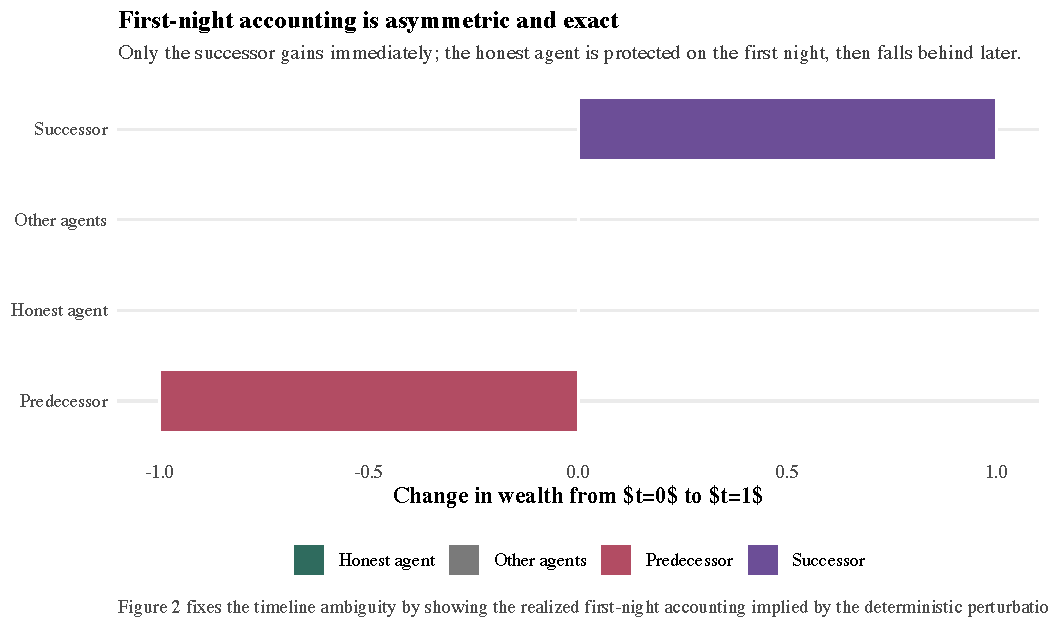
\includegraphics[width=\mediumfigwidth]{figures/fig02_first_night_accounting.pdf}
    \caption{First night accounting. The honest agent is protected on the first night and is robbed only later in the transition, so the winner and loser on that night are the successor and predecessor in the original cycle. This timeline underlies the instability theorem.}
    \label{fig:fig02_first_night_accounting}
\end{figure}

The deterministic environment leaves no room to attribute the departure from the original cycle to chance. Once successor wealth exceeds the threshold in \eqref{eq:threshold}, the continuation path begins to involve further choices to stay home and new interruptions in the network. The event time display therefore traces the mechanism stated in Theorem \ref{thm:no-stationary-one-honest} in realized form.

\subsection{From local asymmetry to class formation}

Longer horizon simulations show that the honest shock generates persistent class structure that survives well beyond the initial reshuffling of positions. Figure \ref{fig:fig03_event_time_roles} groups agents by the highest institutional role they reach during the transition and traces the corresponding wealth paths in event time, a grouping that preserves the early separation because many agents later withdraw into staying or inactivity. Agents who eventually become patrons pull away almost immediately after the initial disturbance, agents who later serve as guards remain well below them, and the honest household falls away sharply. Differentiation therefore begins before the late path settles into a quieter occupational pattern, in line with the theory that rich households emerge first because personal exposure changes the occupational choice of early windfall recipients and patronage enters only after that distribution has already begun to separate.

\begin{figure}[tbp]
    \centering
    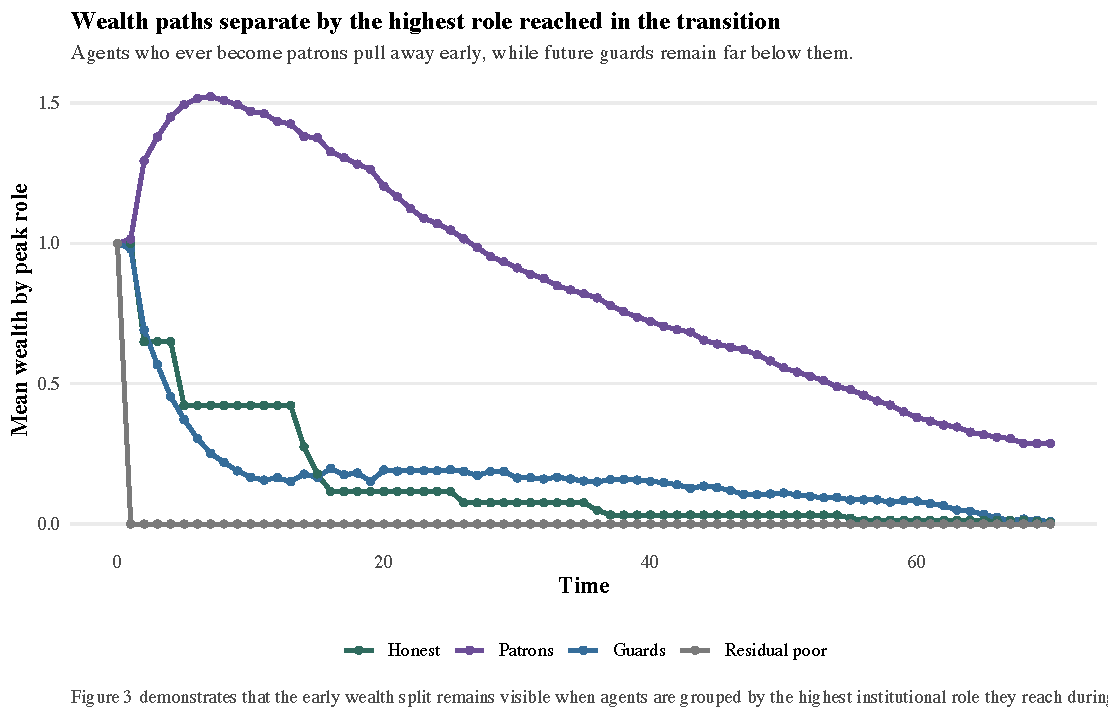
\includegraphics[width=\mainfigwidth]{figures/fig03_event_time_roles.pdf}
    \caption{Event time wealth trajectories by peak role in the transition. Agents who ever become patrons separate quickly from future guards and the residual poor. Class differentiation appears early in the transition and does not depend on the terminal date.}
    \label{fig:fig03_event_time_roles}
\end{figure}

Figure \ref{fig:fig04_distribution_evolution} shows the same process in cross section. The heatmap and quantile ribbons reveal a distribution that rapidly loses its middle. In early periods the support remains narrow because the honest perturbation is still local. A few periods later the upper tail thickens while the lower quantiles bend downward as repeated raids and weak outside options trap a growing mass of agents in the poor set. The widening is not symmetric. The upper tail is carried by a small number of agents who stop exposing their own wealth and later capture part of delegated loot, while the lower tail contains agents who continue to circulate through risky occupations and increasingly depleted target pools. The simulation is therefore producing more than heterogeneity. It is producing a different allocation of risk, power, and occupational choice across the distribution.

\begin{figure}[tbp]
    \centering
    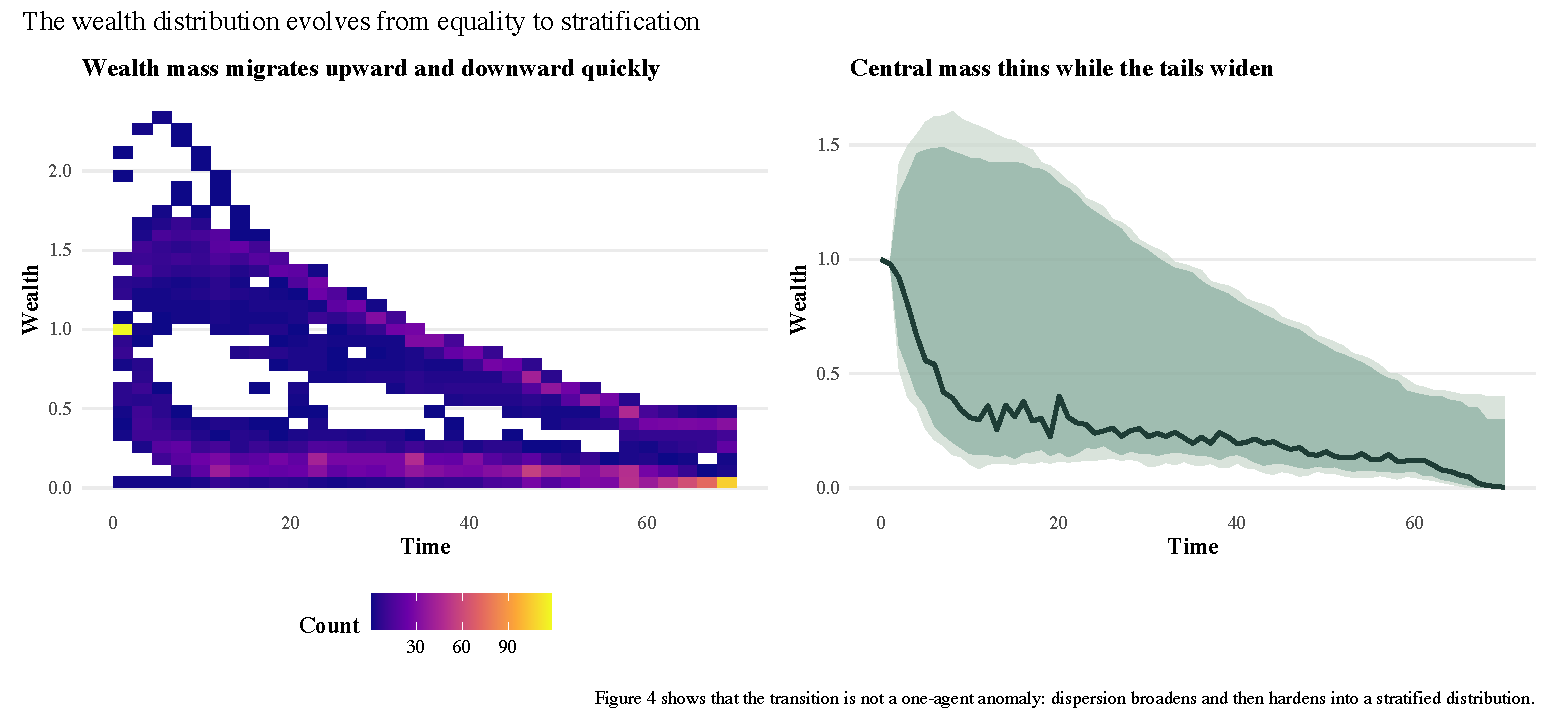
\includegraphics[width=\mainfigwidth]{figures/fig04_distribution_evolution.pdf}
    \caption{Evolution of the wealth distribution. The heatmap and quantile bands show the rapid thinning of the middle and the thickening of both tails. The honest perturbation produces durable stratification instead of a temporary reshuffle.}
    \label{fig:fig04_distribution_evolution}
\end{figure}

Figure \ref{fig:fig05_inequality_dynamics} translates that cross sectional movement into conventional distributional statistics. The Gini coefficient rises sharply from its benchmark value near zero. The top decile wealth share increases in tandem. Lorenz curves at selected dates move steadily away from the forty five degree line. The summary statistics matter because they show that the transition is not confined to a few pathwise anecdotes. The distributional consequences are large, systematic, and persistent in the baseline calibration.

\begin{figure}[tbp]
    \centering
    
\includegraphics[width=\mainfigwidth]{figures/fig05_inequality_dynamics.pdf}
    \caption{Inequality dynamics. The Gini coefficient, top decile wealth share, and Lorenz curves all move sharply away from the egalitarian benchmark. The transition has strong and persistent distributional consequences.}
    \label{fig:fig05_inequality_dynamics}
\end{figure}

These displays show a determinate sequence from local perturbation to durable inequality. The deterministic shock creates a state difference, the exposure threshold turns that difference into differentiated behavior, and the proportional environment amplifies the behavioral split because rich households internalize exposure while poor households remain available for predatory labor. The simulated path therefore gives the theoretical sequence visible economic content instead of leaving it as an abstract transition argument.

\subsection{Patronage and the surplus from delegation}

Across an interpretable range of parameters, rich agents hire poor thieves only when the contract creates surplus that is both feasible and privately valuable. Figure \ref{fig:fig06_contracting_comparative_statics} examines that condition directly. The left panel varies the targeting advantage of delegation. The right panel traces the gap between compensation and the outside option as worker slackness changes. Patron surplus rises with the first margin and falls as the second margin strengthens, exactly as Proposition \ref{prop:patronage} predicts. Delegated theft that is better targeted than freelancing leaves room to satisfy participation and still retain a positive residual. A stronger outside option narrows that residual and can eliminate it.

\begin{figure}[tbp]
    \centering
    
\includegraphics[width=\mainfigwidth]{figures/fig06_contracting_comparative_statics.pdf}
    \caption{Contracting comparative statics. Patron surplus rises when delegated theft has a stronger targeting advantage and poor outside options are weaker. The source of patron surplus is explicit, and the earlier zero profit knife edge disappears.}
    \label{fig:fig06_contracting_comparative_statics}
\end{figure}

Delegation becomes profitable only because the environment generates a clear wedge between delegated returns and the outside option of the thief. If the thief could always obtain alone the same gross loot he could obtain for the patron, and if the patron had neither targeting advantage nor bargaining power, patronage would collapse to a zero-profit transfer. Here the patron directs predation more effectively or protects the contract well enough to make delegation more productive than freelancing, while the thief operates in a crowded and depleted market. The gap between delegated returns and the outside option pays the contracting cost and still leaves a residual for the patron.

Patronage need not be monotone in every parameter that raises expected loot. When theft intensity becomes too large, the prey base can be depleted quickly, which shortens the durability of the contract regime even when delegation is initially attractive. Proposition \ref{prop:patronage} gives the static dominance condition; the simulations trace its interaction with depletion, competition, and regime duration.

\subsection{From patronage to guarding}

Figure \ref{fig:fig07_regime_phase_diagram} maps the dominant medium run regime over the parameter plane spanned by theft intensity and enforcement effectiveness. Low theft intensity combined with weak enforcement tends to preserve a long transition because the returns to both predation and protection remain limited. As theft intensity rises and enforcement becomes more effective, the dominant regime shifts toward coexistence and guarding. Collapse appears where predation is intense enough and protection weak enough that the social base is depleted before a stable protected elite can consolidate. The pattern matches the logic of Theorem \ref{thm:guarding}: once concentrated wealth becomes valuable enough to protect and protection becomes sufficiently effective, elites preserve existing claims instead of financing one more round of delegated extraction.

\begin{figure}[tbp]
    \centering
    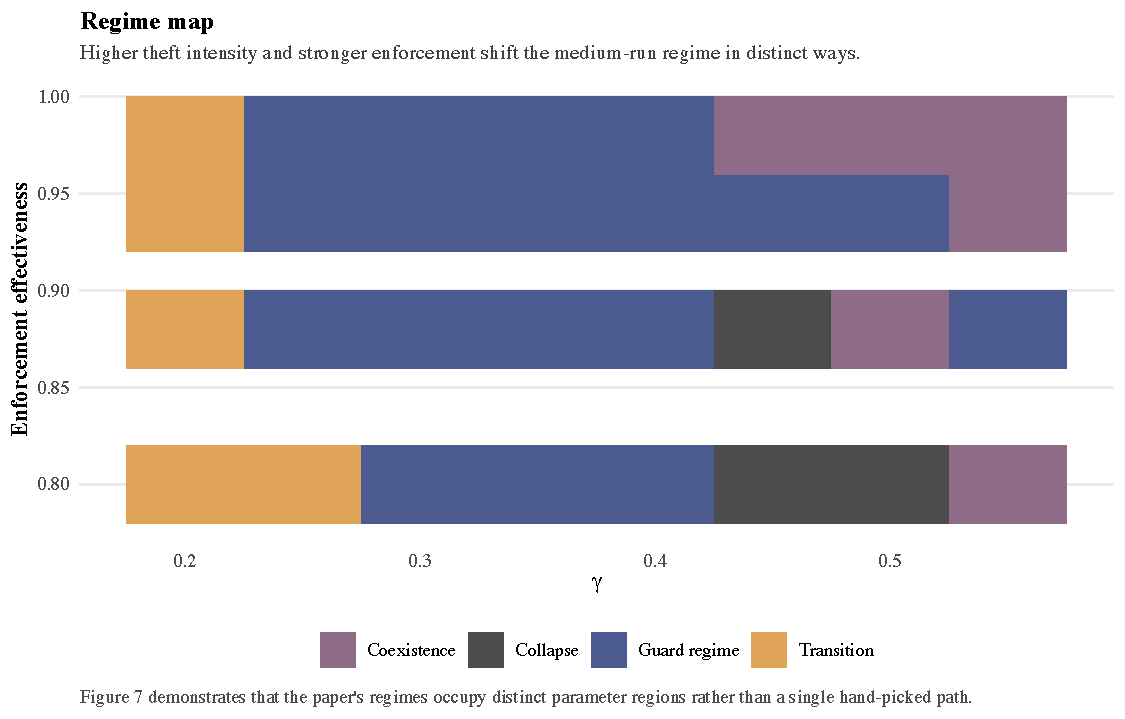
\includegraphics[width=\mediumfigwidth]{figures/fig07_regime_phase_diagram.pdf}
    \caption{Regime phase diagram. Different combinations of theft intensity and enforcement effectiveness lead to distinct medium run transition, coexistence, guard, and collapse regions. The successor regimes occupy distinct and interpretable parts of the parameter space.}
    \label{fig:fig07_regime_phase_diagram}
\end{figure}

On this parameter plane, patronage appears mainly as a transitional corridor and only infrequently as the dominant medium run regime. The diagram is therefore populated mostly by transition, coexistence, guard, and collapse regions, even though patronage remains visible in the event time paths, network snapshots, and contracting comparative statics. The phase diagram adds an important qualification: delegation can organize the middle of the transition without remaining the dominant institutional form once enforcement becomes effective or depletion becomes severe.

Figure \ref{fig:fig08_role_shares} restores time to the same regime logic. The share of agents engaged in direct or freelance theft falls after the first perturbation. Patrons and hired thieves rise next. Guards appear later and remain active through much of the enforcement phase, even though their share is not monotone over time. The plot works as an occupational decomposition of the whole mechanism. The early decline in universal theft reflects the exposure logic of Theorem \ref{thm:no-stationary-one-honest}. The rise in patron and hired thief roles reflects the surplus logic of Proposition \ref{prop:patronage}. The later appearance of guarding reflects the threshold logic of Theorem \ref{thm:guarding}.

\begin{figure}[tbp]
    \centering
    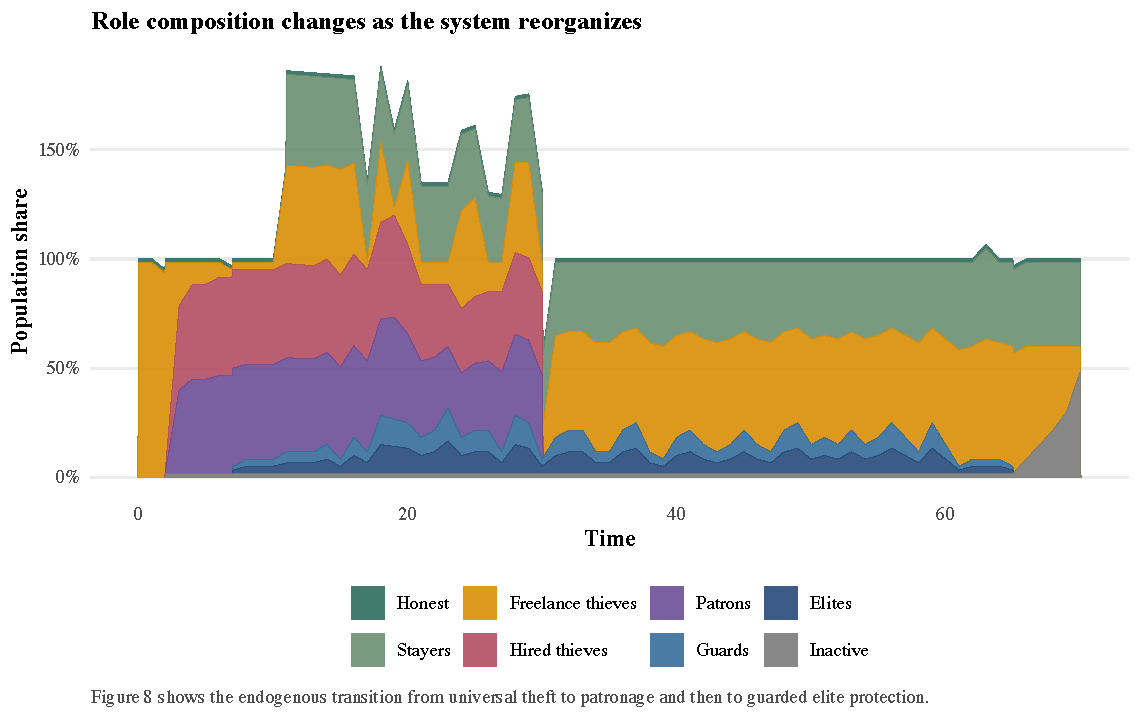
\includegraphics[width=\mainfigwidth]{figures/fig08_role_shares.pdf}
    \caption{Role shares over time. Universal theft gives way first to patronage and later to selective protection, with guarding remaining present through much of the enforcement phase. The social hierarchy reorganizes endogenously after the first honest shock.}
    \label{fig:fig08_role_shares}
\end{figure}

Figure \ref{fig:fig09_transition_timing} separates the part of the transition pinned down by chronology from the part left open by subsequent state evolution. Under the simulation timing, the first opportunity to hire arrives immediately after the deterministic honest shock, and every run generates at least one patron at that first post-shock contracting round, so a raw first-entry statistic for patronage carries little information. The left panel therefore measures the scale of the patronage complex at time $3$, after the first hiring cascade has unfolded, while the right panel records the date at which guards reach five percent of the population. Broader honest shocks do not produce a smooth one for one acceleration in this clustered shock sweep because enlarging the initial honest set changes the local geometry of the broken cycle as well as its size. The picture that remains is immediate reorganization into patronage followed by a later and more dispersed movement into enforcement once wealth concentration and prey depletion have advanced far enough.

\begin{figure}[tbp]
    \centering
    
\includegraphics[width=\mainfigwidth]{figures/fig09_transition_timing.pdf}
    \caption{Early patronage and later guard timing. The first patron appears at the earliest feasible post-shock contracting round in every run, so the left panel reports the share of patrons and hired thieves at time $3$. The right panel reports the time at which guards reach five percent of the population. Organizational change is immediate after the honest shock, while movement into enforcement arrives later and with more dispersion.}
    \label{fig:fig09_transition_timing}
\end{figure}

Coexistence reveals institutional layering instead of a synchronized regime switch. In those paths, some elites have crossed the guard threshold while others still rely on patronage, so different technologies of control operate at the same time in different parts of the wealth distribution. The move from patronage to guarding is therefore unequal and sequential: some elites buy security before others can and stabilize their lead in the process.

Table \ref{tab:simulation-summary} compresses the same sequence across the baseline perturbation, patronage, and enforcement simulations after the timing, regime, and occupational evidence is in place. The baseline perturbation is the least unequal of the three simulated environments. Patronage produces a larger rise in concentration because it adds a contract technology that channels loot upward. Enforcement then preserves and slightly intensifies that concentration. In this sense the table mirrors Proposition \ref{prop:welfare}: distributional divergence is already visible once reciprocity breaks, and later regimes magnify that divergence or lock it in through new organizational choices.

\begin{table}[tbp]
    \centering
    \caption{Simulation summary. The first honest perturbation produces a local distributional break, patronage transforms that break into durable stratification, and enforcement preserves or deepens concentrated wealth instead of reversing it.}
    \label{tab:simulation-summary}
    \begin{tabular}{lcccll}
\toprule
Scenario & Gini & Top decile & First patron & First guard & Regime \\
\midrule
Baseline perturbation & 0.231 & 0.200 & Not reached & Not reached & Transition \\
Patronage dynamics & 0.575 & 0.296 & 2 & Not reached & Transition \\
Enforcement dynamics & 0.640 & 0.306 & 2 & 7 & Guard regime \\
\bottomrule
\end{tabular}

\end{table}

\subsection{Network reorganization and welfare}

Figure \ref{fig:fig10_network_snapshots} makes the organizational change visible in network form. On the first honest night the graph is still dominated by direct theft edges arranged around the original cycle. In the middle snapshot, contract links connect patrons to hired thieves and theft edges point from those thieves toward vulnerable poor households. In the later snapshot, guard links radiate from elite households while direct theft edges thin out. The pattern of social linkage changes along with the wealth distribution, as horizontal predation gives way to vertical contracting and then to selective protection.

\begin{figure}[tbp]
    \centering
    
\includegraphics[width=\mainfigwidth]{figures/fig10_network_snapshots.pdf}
    \caption{Network snapshots across regimes. Direct theft edges dominate at first, contract edges later connect patrons to thieves, and guard edges eventually organize elite protection. The network structure of predation and control changes with the regime.}
    \label{fig:fig10_network_snapshots}
\end{figure}

Figure \ref{fig:fig11_welfare_decomposition} reports the welfare consequences of the transition. Gross wealth and utilitarian welfare do not move together. Aggregate wealth declines steadily because theft, punishment, and protection burn resources even when much of the interaction is redistributive in form. Welfare deteriorates more sharply because redistribution toward the top lowers the concave utility sum and because predation, contracting, punishment, and guarding all consume resources. Proposition \ref{prop:welfare} formalizes this mechanism. Low welfare in the transition comes from the unequal and resource consuming adjustment that follows an incomplete honest shock.

\begin{figure}[tbp]
    \centering
    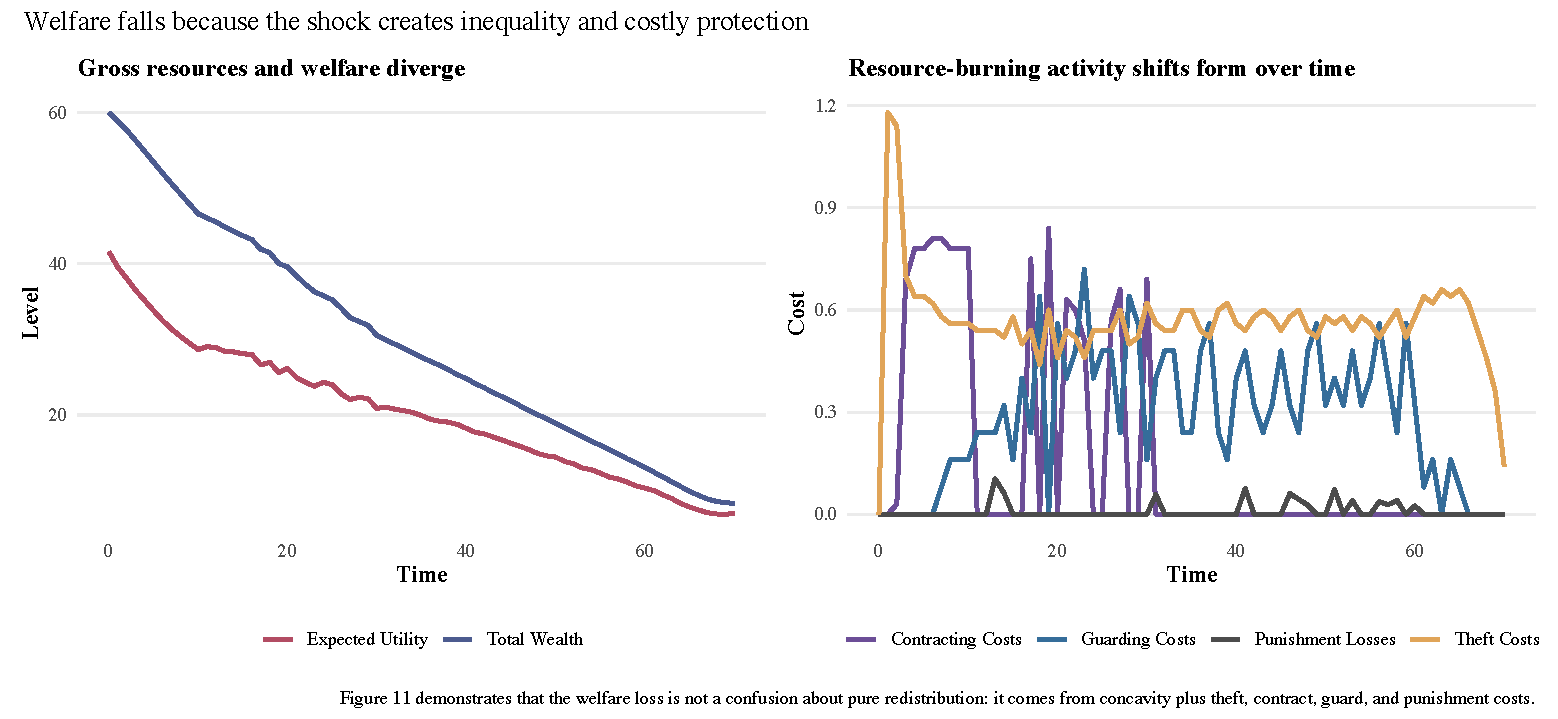
\includegraphics[width=\mainfigwidth]{figures/fig11_welfare_decomposition.pdf}
    \caption{Welfare decomposition. Aggregate wealth and utilitarian welfare diverge because the transition adds inequality and resource burning activity in the form of theft, contracts, punishment, and guarding. The welfare mechanism appears directly in the decomposition.}
    \label{fig:fig11_welfare_decomposition}
\end{figure}

Because Figure \ref{fig:fig11_welfare_decomposition} follows one baseline enforcement path rather than a comparison across parameter regions, its most direct contribution lies in the composition of resource use over time. Theft costs dominate early, contracting costs spike during patronage, and guarding costs remain persistent later on. Guard adoption changes how resources are burned without restoring the earlier welfare level, and the protected order that emerges at the end still rests on concentrated wealth accumulated during the predatory transition.

\subsection{Robustness}

Figure \ref{fig:fig12_robustness_panels} collects the main one dimensional robustness exercises in compact form. Final welfare responds most strongly to theft intensity and occupied house vulnerability in this sweep, while final inequality moves within a narrower band. Regime classification also changes little once the system is already in the region where guarding is attractive. Among the four margins shown, only the theft intensity sweep changes the dominant regime, passing from transition to guard and then to coexistence as extraction becomes harsher. The other sweeps mainly alter the severity of the outcome. The panels therefore indicate a mechanism that survives beyond a single calibration, even though some margins move welfare far more than they move regime labels.

\begin{figure}[tbp]
    \centering
    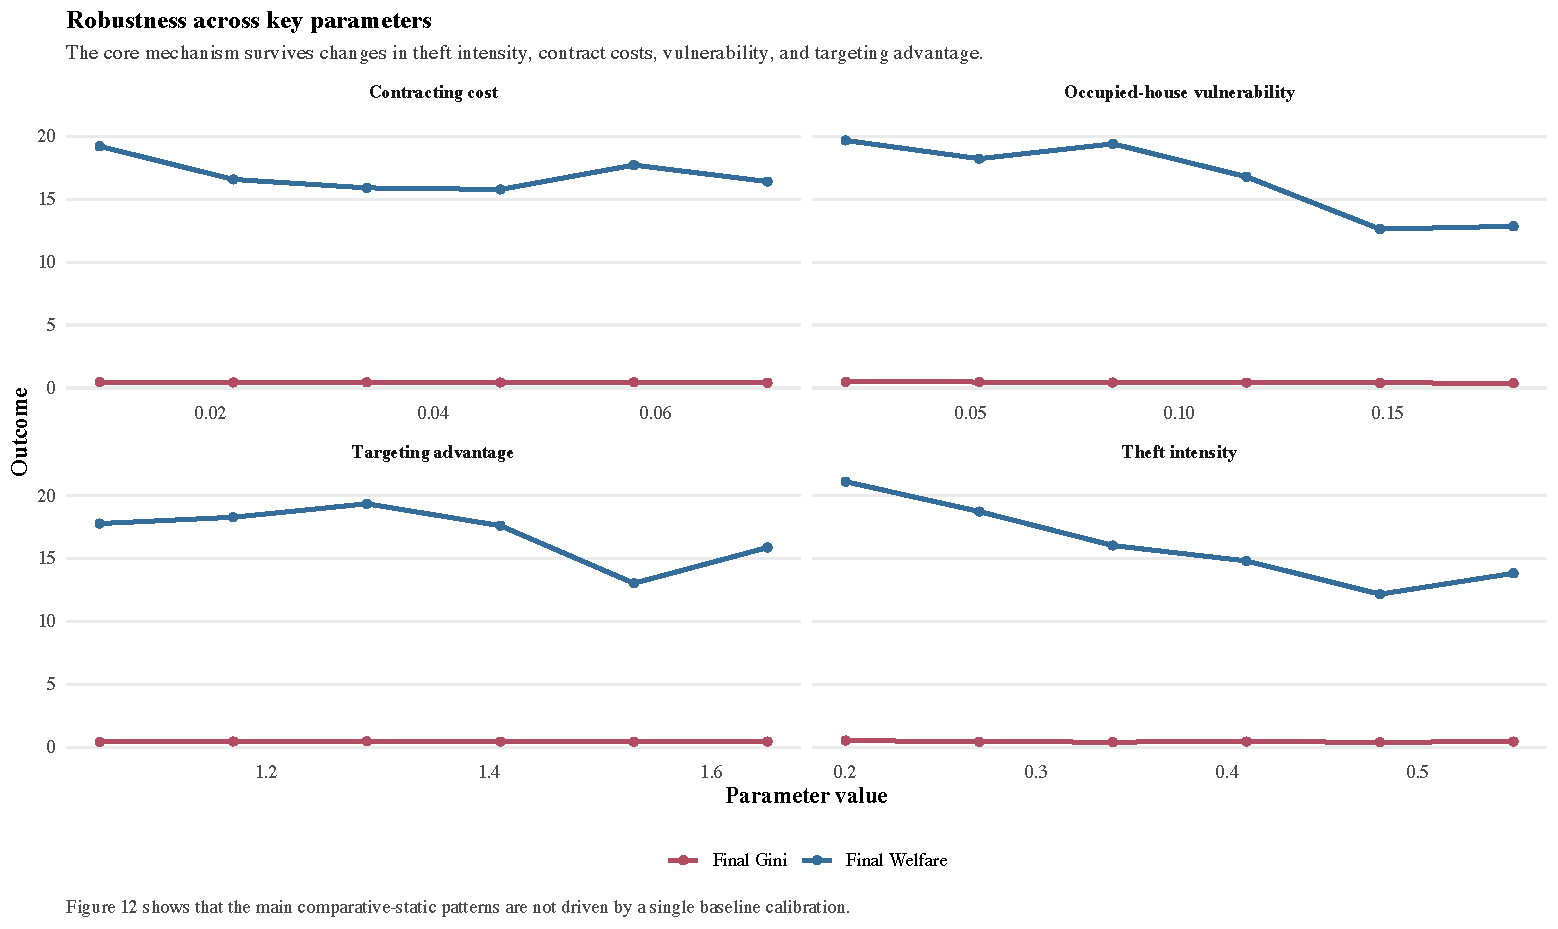
\includegraphics[width=\mainfigwidth]{figures/fig12_robustness_panels.pdf}
    \caption{Robustness panels. The top row reports final inequality, the bottom row reports final welfare, and point markers identify the dominant regime reached at each parameter value. The mechanism survives beyond a single calibration, although some margins move welfare more than regime labels.}
    \label{fig:fig12_robustness_panels}
\end{figure}

The failure cases identify the conditions under which the mechanism attenuates. High contracting costs and weak targeting advantage compress delegation surplus, while low occupied house vulnerability reduces the value of moving from mere presence to organized protection. The sweeps therefore locate the margins that mute the transition without suggesting that every one dimensional variation redraws the institutional map.

Figure \ref{fig:fig07_regime_phase_diagram} is the more informative display for collapse. There the collapse cells do not mark a numerical artifact or a moral inversion of balanced reciprocity. They identify paths in which predation and protection together destroy the social base that made them profitable. Poor households become too depleted to sustain patronage, and inequality becomes so sharp that a small protected core cannot reorganize the rest into a stable order. This possibility prevents the model from telling a falsely deterministic story in which every corrupt equilibrium matures smoothly into guarded hierarchy.
